\PassOptionsToPackage{x11names}{xcolor}
\documentclass[10pt]{beamer}
\usetheme[
%%% option passed to the outer theme
%    progressstyle=fixedCircCnt,   % fixedCircCnt, movingCircCnt (moving is deault)
  ]{Feather}
  
% If you want to change the colors of the various elements in the theme, edit and uncomment the following lines

% Change the bar colors:
%\setbeamercolor{Feather}{fg=red!20,bg=red}

% Change the color of the structural elements:
%\setbeamercolor{structure}{fg=red}

% Change the frame title text color:
%\setbeamercolor{frametitle}{fg=blue}

% Change the normal text color background:
%\setbeamercolor{normal text}{fg=black,bg=gray!10}

%-------------------------------------------------------
% INCLUDE PACKAGES
%-------------------------------------------------------
%\usepackage{fourier, heuristica}
%\usepackage{tgadventor}
\usepackage{array,booktabs}
\usepackage{graphicx}
\usepackage{colortbl,xcolor}
\usepackage{caption}
\usepackage{amsmath,mathrsfs}
\usepackage{verbatim}
\usepackage{stackrel,stackengine}
\usepackage{ragged2e}
\usepackage{pgf,tikz}
\usepackage{multimedia}
\usepackage{media9}
\usepackage{listings}  % Agrega color al código de un lenguaje de programación
%------------------------------------------------------
%\usepackage[utf8]{inputenc}
%\usepackage[T1]{fontenc}
\usepackage[spanish]{babel}
\usepackage{fontspec}
\setmainfont{AncizarSans-Regular.otf} 
\usepackage[ruled,vlined,lined,linesnumbered,algosection,english]{algorithm2e} %

%-------------------------------------------------------
% DEFFINING AND REDEFINING COMMANDS
%-------------------------------------------------------
\DeclareCaptionFont{blue}{\color{black}}
\newcommand{\foo}{\color{red}\makebox[0pt]{\textbullet}\hskip-0.5pt\vrule width 1.3pt\hspace{\labelsep}}

%--------------------------------------------------------
\renewcommand\useanchorwidth{T}
\def\theyearwidth{1.5pt}
\newlength\yrsfboxrule
\yrsfboxrule .4\fboxrule
\newcommand\yearwidth[1]{\def\theyearwidth{#1}\ignorespaces}
\newcommand\skipyears[2][white]{%
  \fboxrule\yrsfboxrule%
  \fboxsep=-\yrsfboxrule%
  \fcolorbox{gray}{#1}{\strut\hspace{#2}}%
  \ignorespaces%
}
\newcommand\showyear[2][black]{%
  \fboxsep=0pt%
  \stackon{%
    \colorbox{#1}{\strut\hspace{\theyearwidth}}%
  }{\sffamily\small#2}%
  \ignorespaces%
}

%-----------------------------------------------------------
% colored hyperlinks
\newcommand{\chref}[2]{
  \href{#1}{{\usebeamercolor[bg]{Feather}#2}}
}

%-------------------------------------------------------
% INFORMATION IN THE TITLE PAGE
%-------------------------------------------------------

\title[] % [] is optional - is placed on the bottom of the sidebar on every slide
{ % is placed on the title page
      \textbf{Modelo de direccionamiento IPv6 para redes Ad-hoc basadas en comunicaciones tipo máquina a máquina}
}

\subtitle[Grupo de Investigación en Redes de Telecomunicaciones Dinámicas \& Lenguajes de Programación Distribuidos]
{
      %\textbf{Avance 4 - Implementación y simulación}
}

\author[TLÖN]
{   
    Giuseppe Roa Osorio \\
    {\ttfamily groao@unal.edu.co}\\
    Candidato a MsC Telecomunicaciones\\
    \vspace{0.5cm}
    Director: PhD Jorge Eduardo Ortiz\\
    {\ttfamily jeortizt@unal.edu.co}
}

\institute[]
{
    \large{Universidad Nacional de Colombia}\\
    \small{Sede Bogotá - Facultad de Ingeniería\\
    Departamento de Ingeniería de Sistemas e Industrial}
  
  %there must be an empty line above this line - otherwise some unwanted space is added between the university and the country (I do not know why;( )
}

%\date{\today}
\date{7 de Octubre de 2019}

%-------------------------------------------------------
% THE BODY OF THE PRESENTATION
%-------------------------------------------------------

\begin{document}

\setbeamertemplate{caption}[numbered] % Enable tables/figures numbering
%-------------------------------------------------------
% THE TITLEPAGE
%-------------------------------------------------------

{\1% % this is the name of the PDF file for the background
\begin{frame}[plain,noframenumbering] % the plain option removes the header from the title page, noframenumbering removes the numbering of this frame only
  \titlepage % call the title page information from above
\end{frame}}

%-------------------------------------------------------

\begin{frame}{Agenda}{}
\tableofcontents
\end{frame}

%-------------------------------------------------------

	%-------------------------------------------------------
\section{Contexto - Motivación}
%-------------------------------------------------------
%\subsection{Motivación}
\begin{frame}{Ecosistema de dispositivos}{Contexto - Motivación}
%-------------------------------------------------------
    \begin{figure}				
		{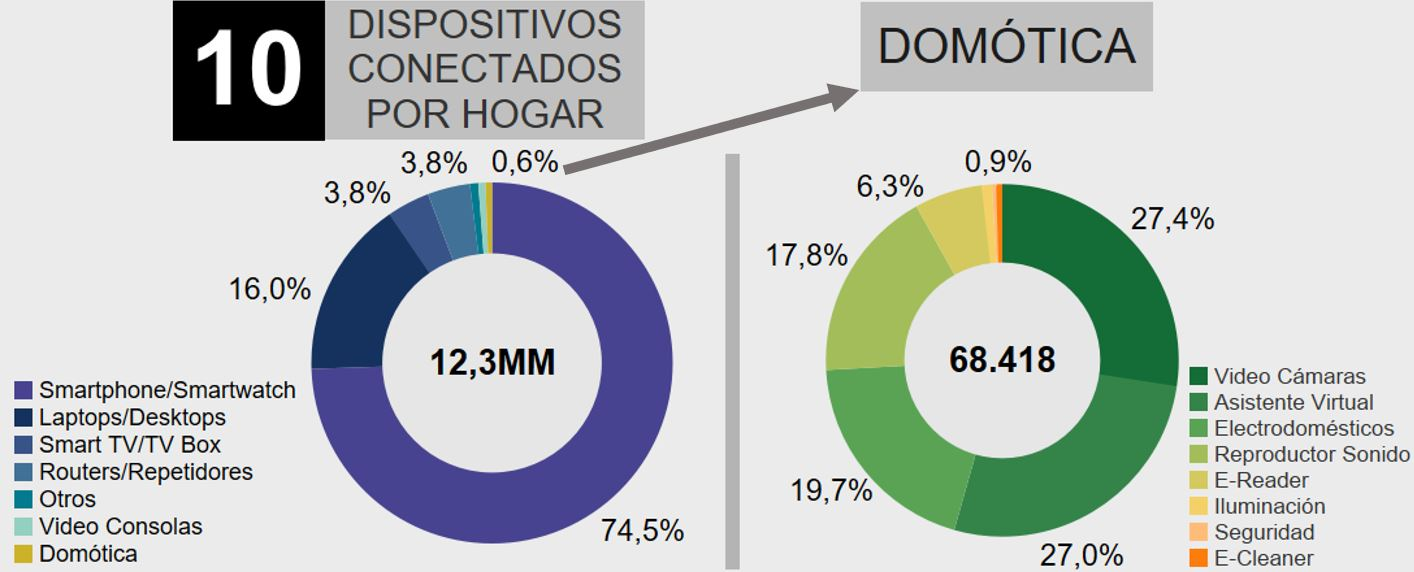
\includegraphics[width=0.99\textwidth,keepaspectratio]{Sustentacion/Figures/DispositivosColombia.JPG}}
		\caption{\small \sl Dispositivos en el mercado colombiano [Fuente Propia]}
		\label{figure:Ecosistema}
    \end{figure}
\end{frame}
%-------------------------------------------------------
\begin{frame}{Comunicaciones M2M}{Contexto - Motivación}
%-------------------------------------------------------
\begin{figure}[htbp]
	    \centering
		\fbox{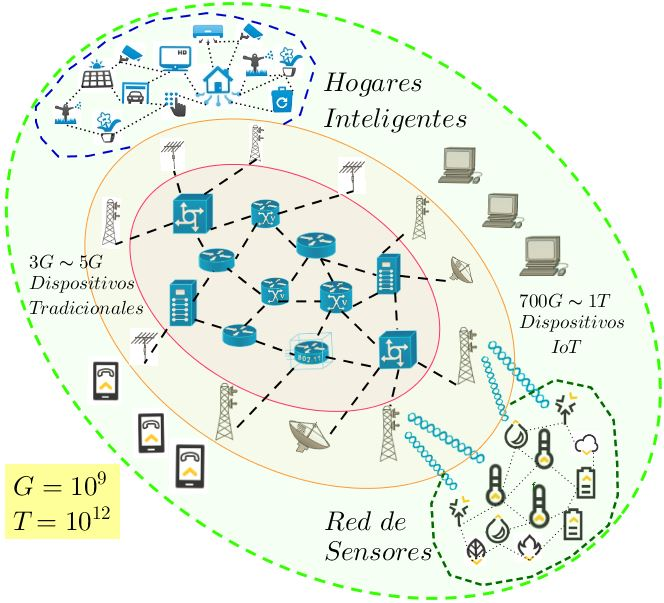
\includegraphics[height=0.7\textheight,keepaspectratio]{Figures/M2M.JPG}}
	    \caption{Comunicaciones M2M \cite{DoWeNeed}}
	    \label{fig:M2M}
    \end{figure}
\end{frame}
%-------------------------------------------------------
\begin{frame}{Paradigma M2M}{Contexto - Motivación}
%-------------------------------------------------------
\begin{block}{Cambio de paradigma}
  \begin{itemize}
    \justifying
    \item<1-|alert@1> Actualmente la industria esta experimentando un crecimiento sin precedentes de sensores y actuadores simples fabricados por diversos proveedores y limitados en recursos computacionales \cite{M2MARCHITECTUREPERFORMANCE}. 
    \item<2-|alert@2> Gestionar y analizar los importantes volúmenes de información, en gran medida redundante, es un reto técnico en las redes actuales \cite{IOTIPV6MIPV6}.
    \item<3-|alert@3> Minimizar los costos acumulados en Hadware/Software, Vigilancia, Gestión y Seguridad es un factor clave en el despliegue del IoT \cite{RethinkIOT}.
    \item<4-|alert@4> No existen arquitecturas de redes de comunicaciones humanas que se adecuen al tamaño del IoT \cite{RethinkIOT}. 
  \end{itemize}
 \end{block}
\end{frame}
%-------------------------------------------------------
%\subsection{Características Generales}
\begin{frame}{Dinámica de red}{Contexto - Motivación}
%-------------------------------------------------------
    \begin{figure}[htbp]
	    \centering
		\fbox{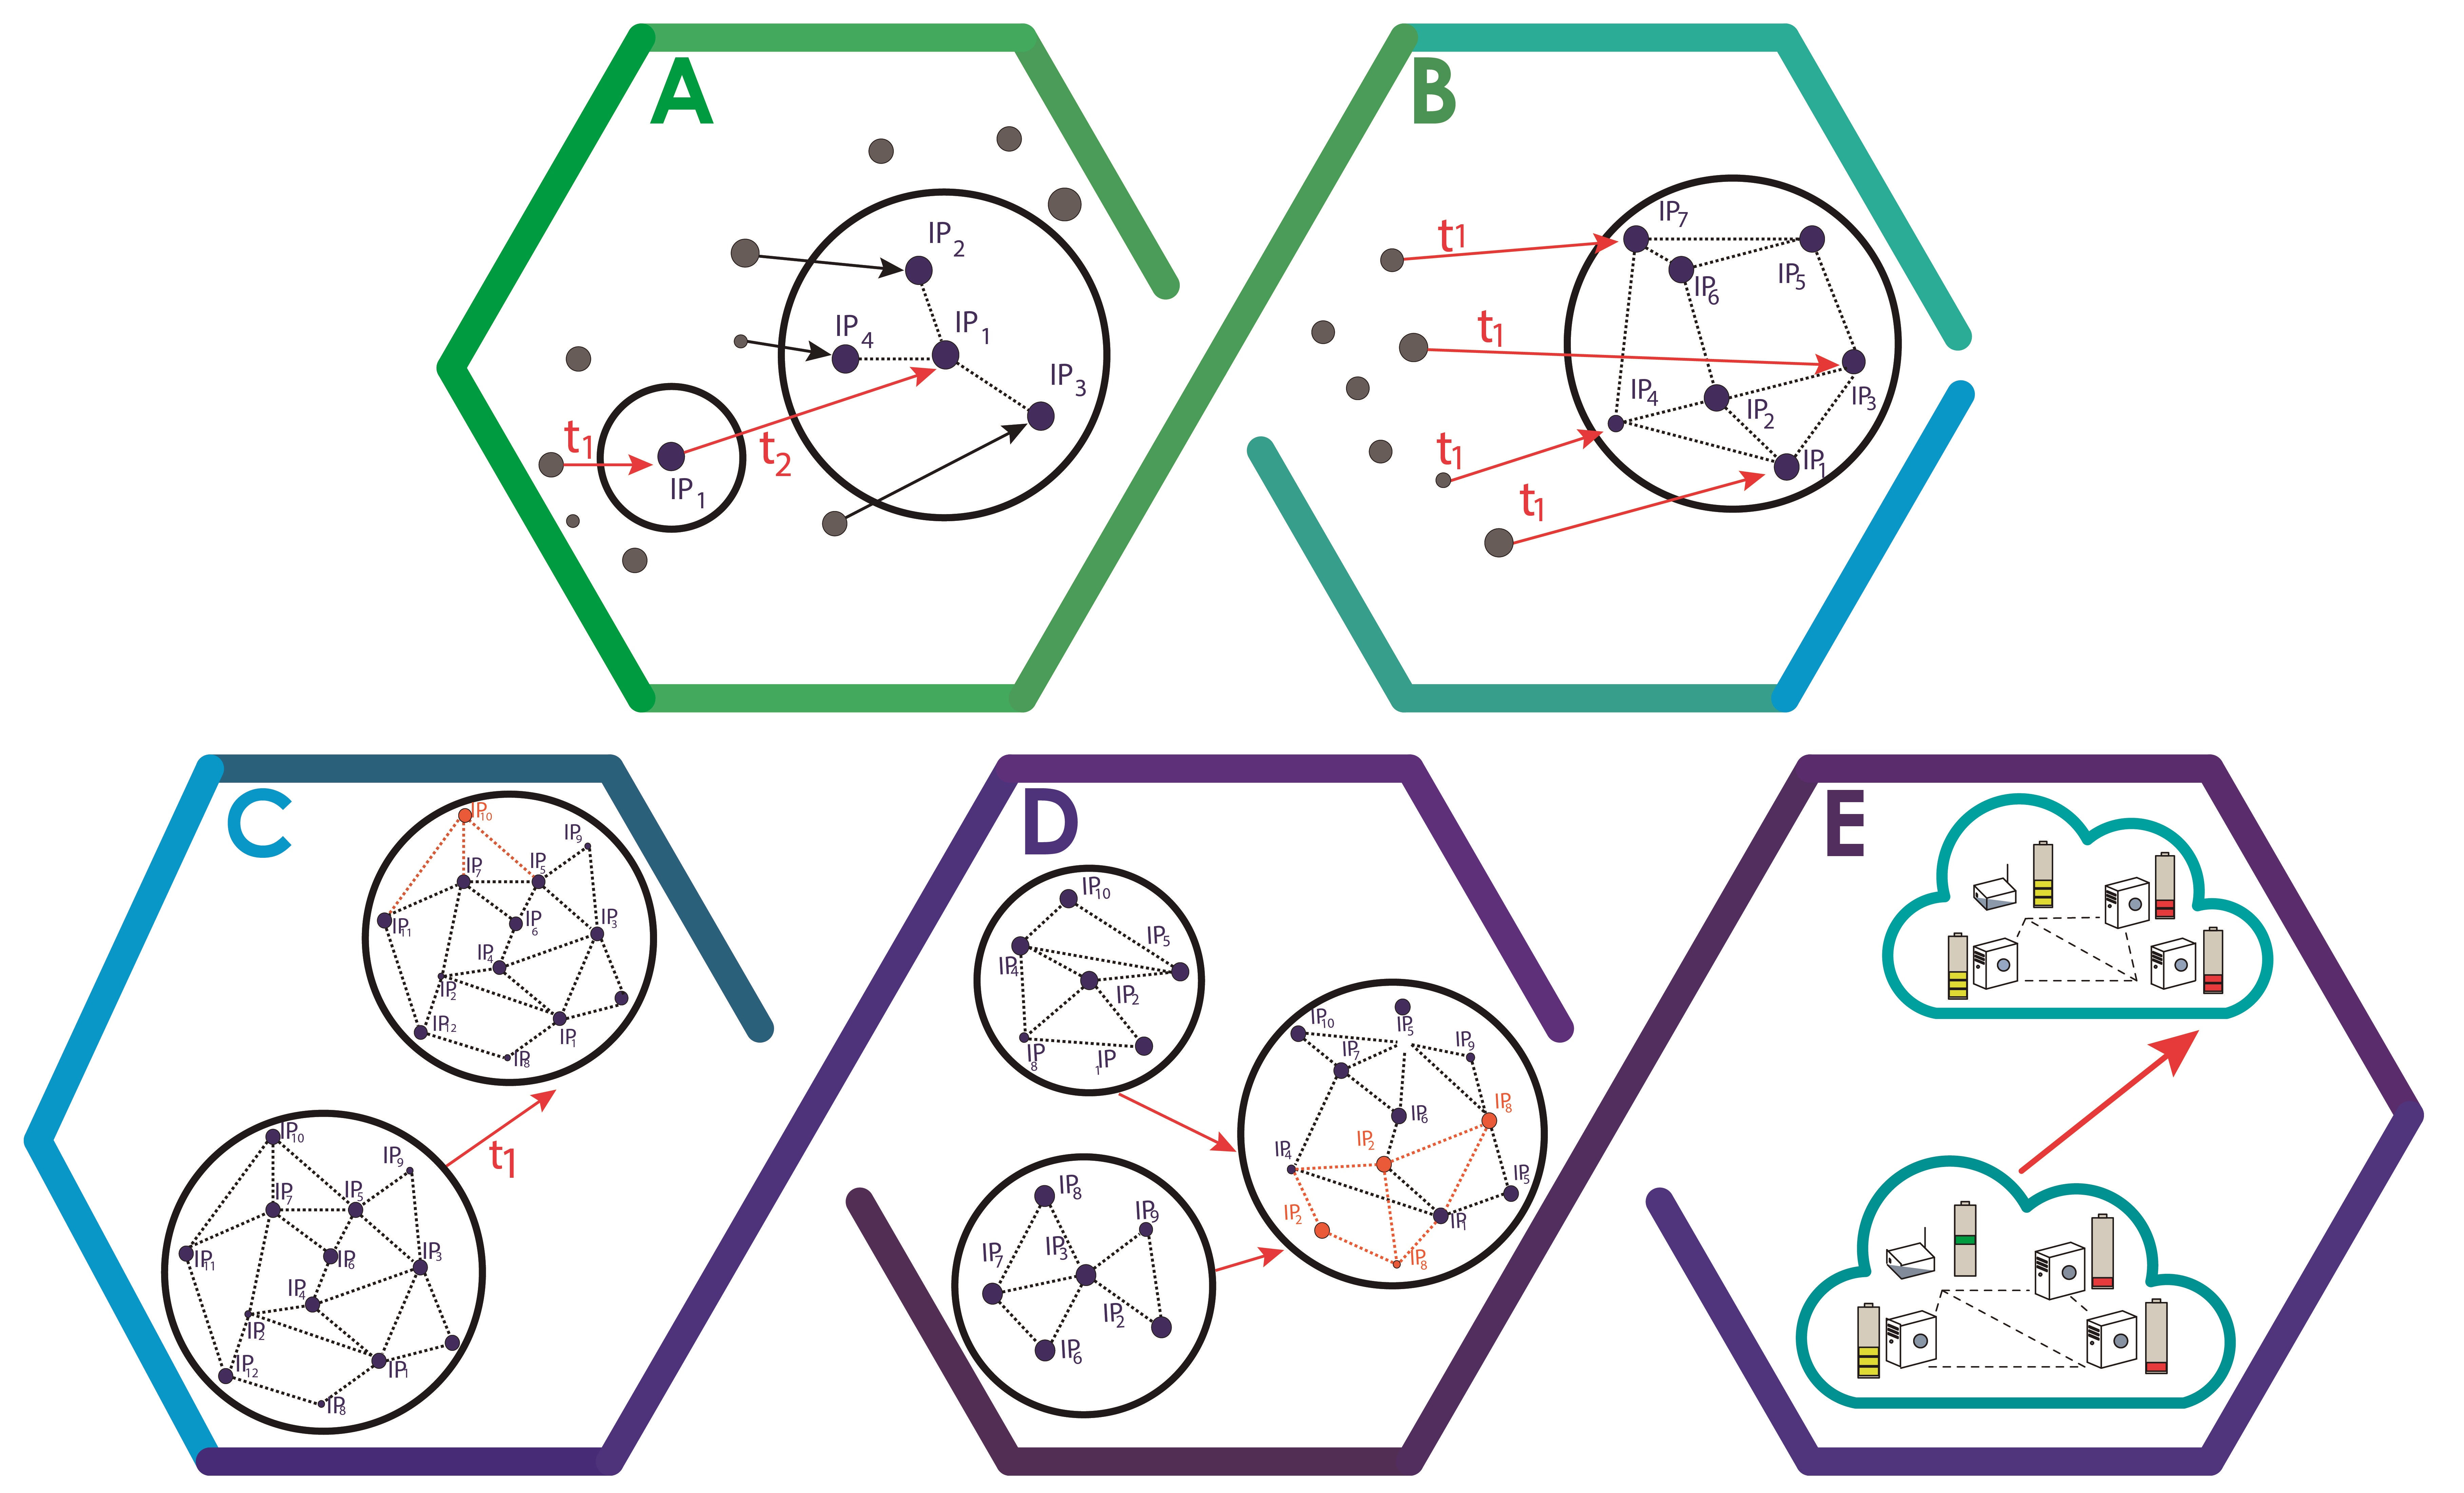
\includegraphics[height=0.65\textheight,keepaspectratio]{Figures/DinamicaManets.jpg}}
	    \caption{Dinámica de las MANETs [Fuente propia]}
	    \label{fig:DinMan}
    \end{figure}
\end{frame}
%-------------------------------------------------------
%\subsection{Marco Conceptual}
%\begin{frame}{Contexto}{Marco Conceptual \cite{DATMANET}}
%-------------------------------------------------------
%\begin{block}{Requerimientos protocolo de direccionamiento}
%  \begin{itemize}
%    \justifying
%    \item Cada nodo debe obtener una dirección IP dinámicamente.
%    \item En ningún instante del tiempo deberían haber IP's %duplicadas.
%    \item Cuando un nodo ''abandone'' la red, la IP debe ser liberada.
%    \item Cuando se efectué una migración de redes el esquema debe detectar y corregir duplicidades. 
%    \item El protocolo debe asegurar que solo nodos autorizados pueden tener acceso a los recursos. 
%    \item El esquema debe ser tolerante a fallas en los nodos.
%    \item Se deben minimizar los paquetes señalización. 
%  \end{itemize}
% \end{block}
%\end{frame}

	%-------------------------------------------------------
\section{Problema - Objetivos - Producción}
%-------------------------------------------------------
\subsection{Pregunta de Investigación}
\begin{frame}{Problema y Objetivos}{Pregunta de Investigación}
%-------------------------------------------------------
  \begin{block}{Problema de Investigación}
   \begin{itemize}
   \justifying
    \item<1->  ¿Cómo realizar el direccionamiento de dispositivos heterogéneos conectados en una red Ad-Hoc, basada en comunicaciones máquina a máquina, autoconfigurable independientemente de la cantidad de dispositivos involucrados? 
    \item<1->  Los procesos y técnicas a emplear deberán estar enfocadas a la escalabilidad, simplicidad y robustez deseada en implementaciones encaminadas a servicios con conexiones tipo máquina-máquina.
    \end{itemize}
  \end{block}
\end{frame}
%-------------------------------------------------------
\subsection{Objetivos}
\begin{frame}{Problema y Objetivos}{Objetivos}
%-------------------------------------------------------
  \begin{block}{Objetivo General}
    \begin{itemize}    
    \item Diseñar un modelo de direccionamiento IPv6 en redes Ad-Hoc basadas en comunicaciones tipo máquina-máquina. 
    \end{itemize}
  \end{block}
  %\pause
  \begin{block}{Objetivos Específicos}
    \begin{itemize}
    \justifying
        \item Modelar los principales requerimientos en la asignación de direcciones IPv6 para redes Ad-Hoc.
        \item Adaptar, mediante técnicas bio-inspiradas, un algoritmo clásico de asignación dinámica de direcciones IPv6 para una red Ad-Hoc de 10 nodos. 
        \item Definir tres métricas representativas acerca del desempeño, sensibles para el modelo de direccionamiento propuesto.
    \end{itemize}
  \end{block}
\end{frame}
%-------------------------------------------------------
\begin{frame}{Problema y Objetivos}{Objetivos} 
  \begin{block}{Objetivos Específicos}
    \begin{itemize}
    %\setcounter{enumi}{3}
    \justifying
        \item Diseñar al menos tres escenarios de simulación en un software determinado, para someter el modelo de direccionamiento a diferentes condiciones a las que se podría enfrentar en una implementación real.
        \item Evaluar el desempeño del modelo planteado mediante simulaciones analizando las métricas definidas durante la ejecución de la tesis.
    \end{itemize}
  \end{block}
\end{frame}
%-------------------------------------------------------
\subsection{Producción Académica}
\begin{frame}{Problema y Objetivos}{Producción Académica}
%-------------------------------------------------------}
\centering

\includegraphics[width=0.7\textwidth,height=0.7\textheight,keepaspectratio]{Figures/COLCACI.JPG}\\

\includegraphics[width=0.6\textwidth,height=0.6\textheight,keepaspectratio]{Figures/CICOM.JPG}
\end{frame}
	%-------------------------------------------------------
\section{Modelo Propuesto}
%-------------------------------------------------------
\subsection{Modelos Bio-inspirados / Social-inspirados}
\begin{frame}{Modelos Bio-inspirados - Distribución de Polen}{Modelo Propuesto}
%-------------------------------------------------------
    \begin{figure}				
		\fbox{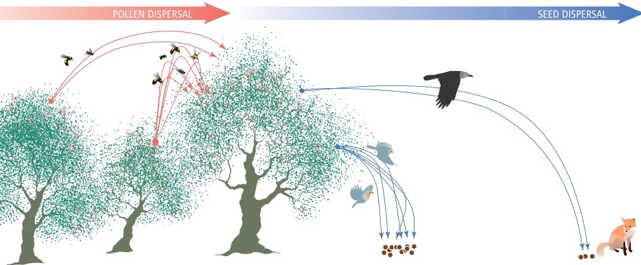
\includegraphics[width=\textwidth,keepaspectratio]{Figures/Pollen.PNG}}
		\caption{\small \sl Distribución de Polen \cite{pollen}}
		\label{figure:Pollen}
    \end{figure}
\end{frame}
%-------------------------------------------------------
\begin{frame}{Modelos Bio-inspirados- Inteligencia de Enjambres}{Modelo Propuesto}
%-------------------------------------------------------
    \begin{figure}				
		\fbox{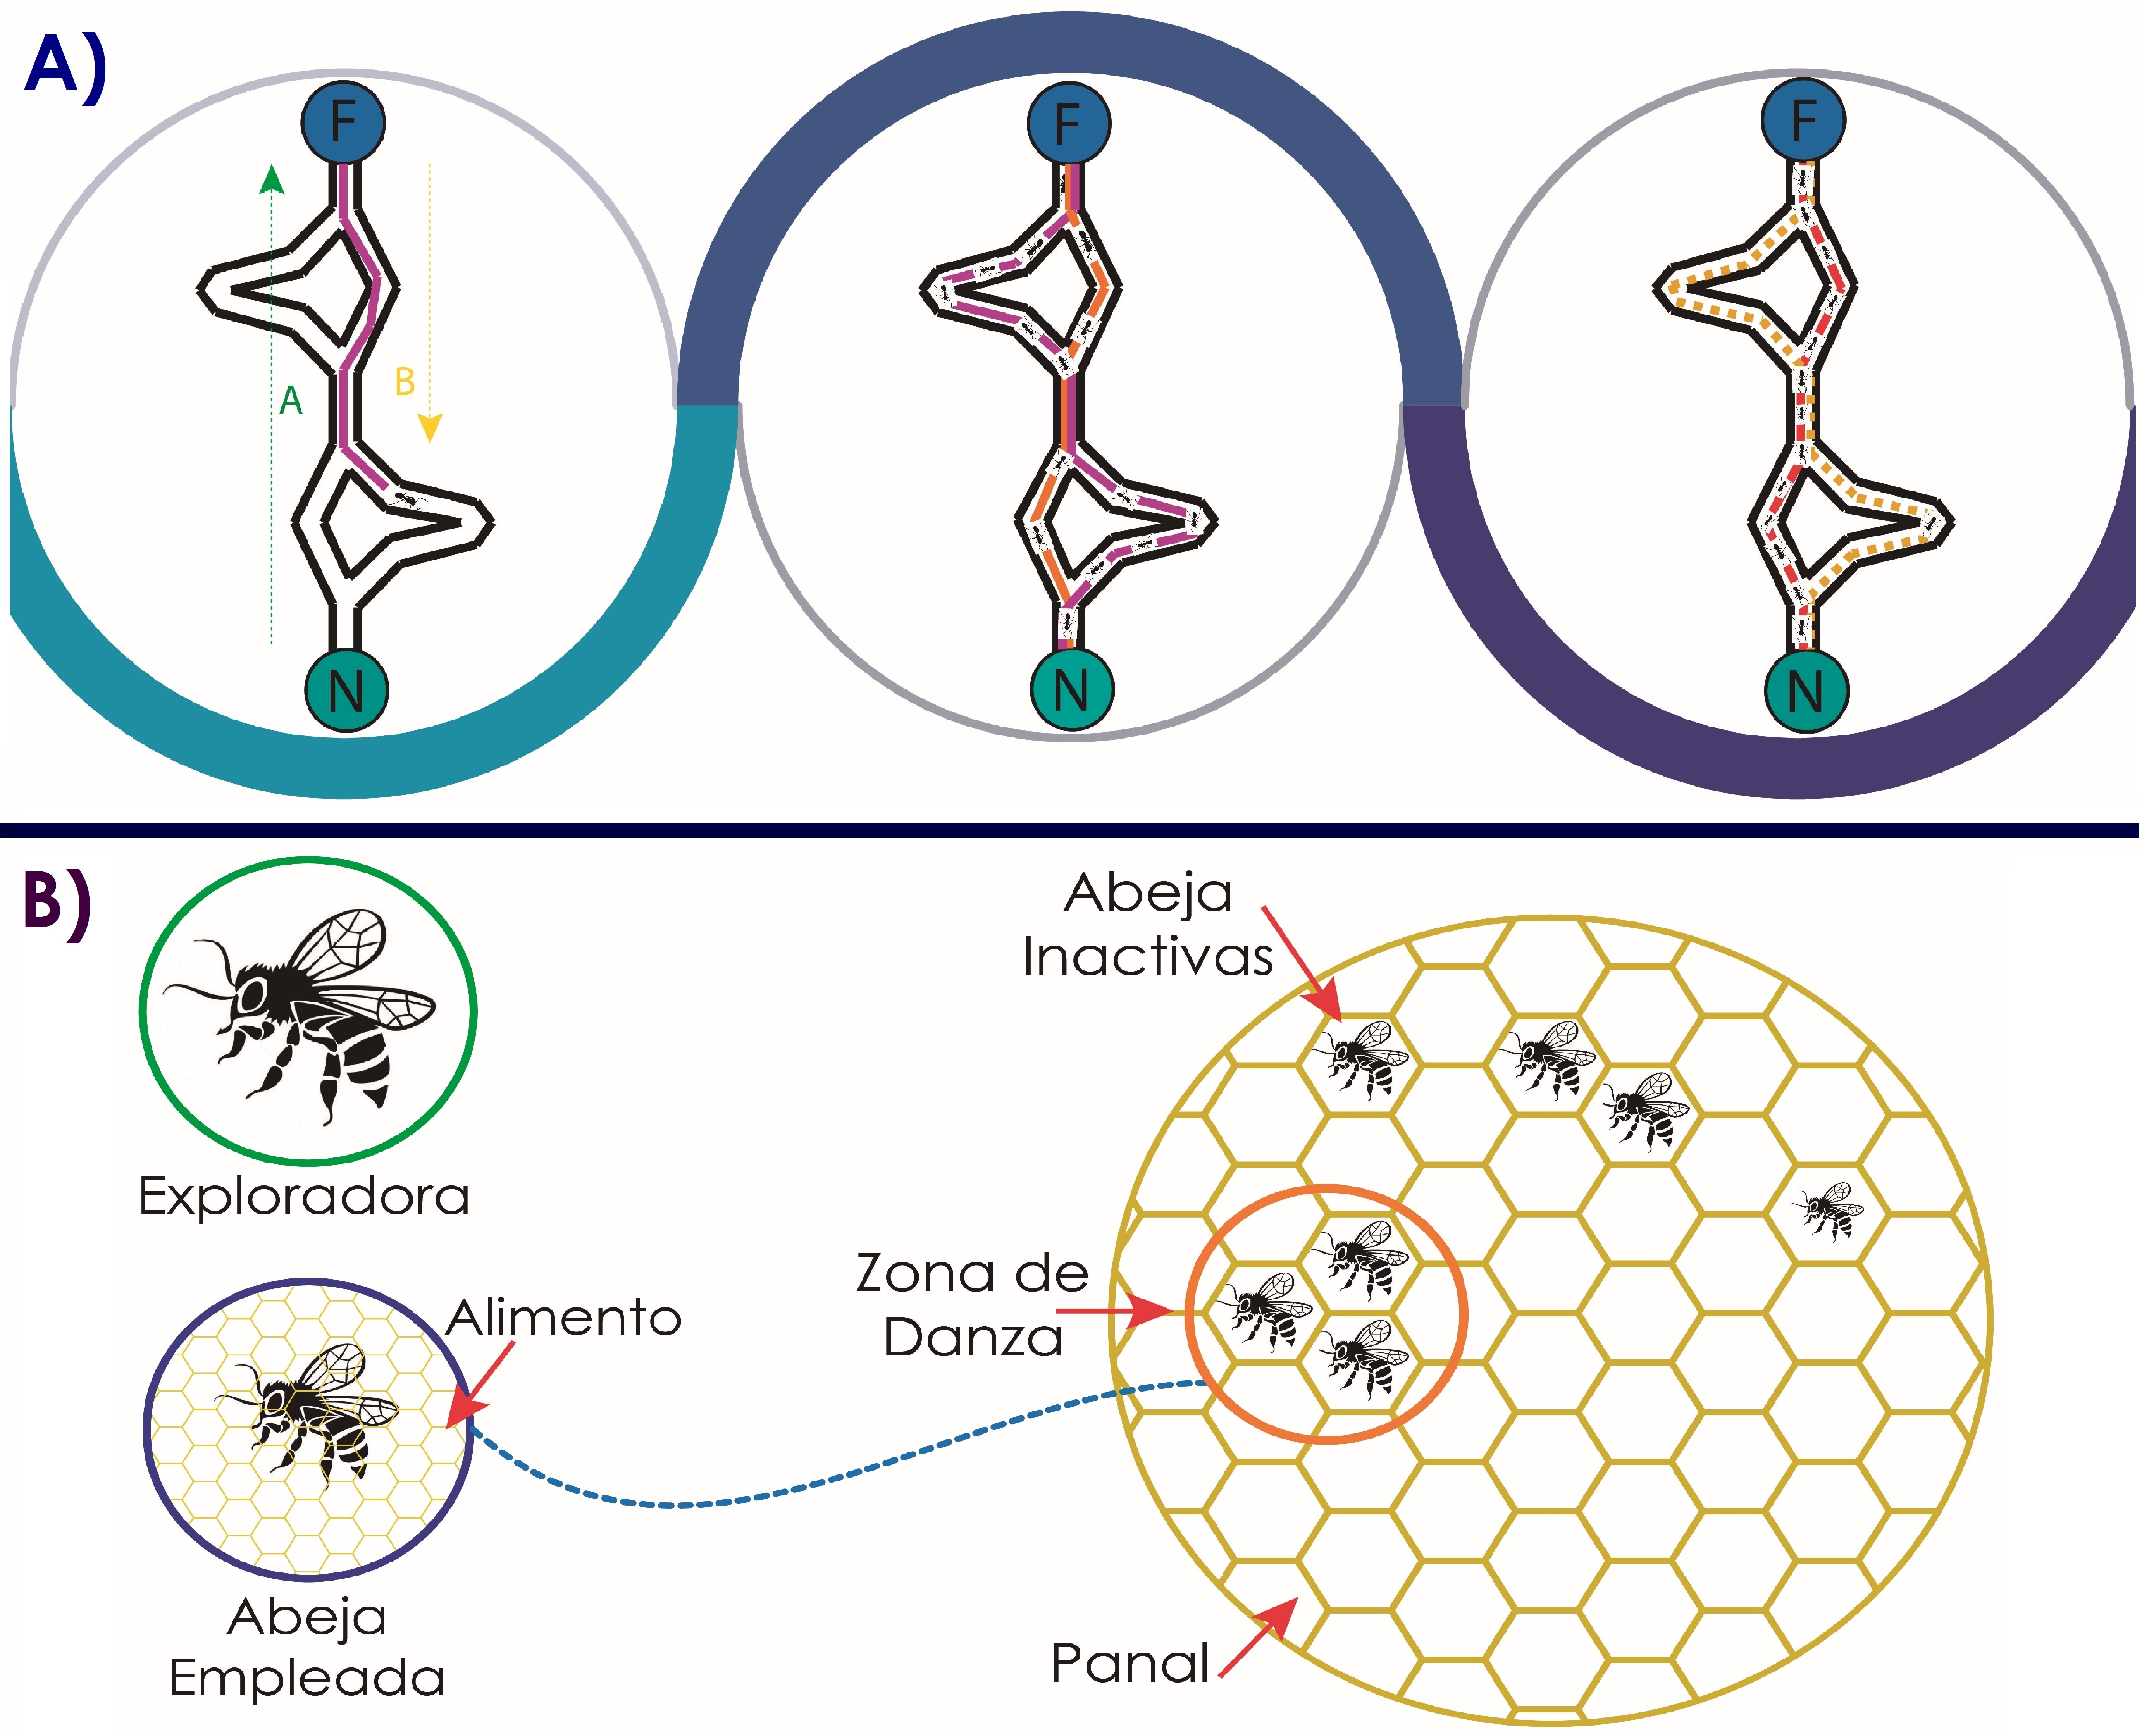
\includegraphics[height=0.7\textheight,keepaspectratio]{Figures/ants-bees.jpg}}
		\caption{\small \sl Inteligencia de Enjambres\cite{chanPSO}}
		\label{figure:Swarm}
    \end{figure}
\end{frame}
%-------------------------------------------------------
\begin{frame}{Modelos Social-inspirados- Modelo TLÖN}{Modelo Propuesto}
%-------------------------------------------------------
    \begin{figure}				
		\fbox{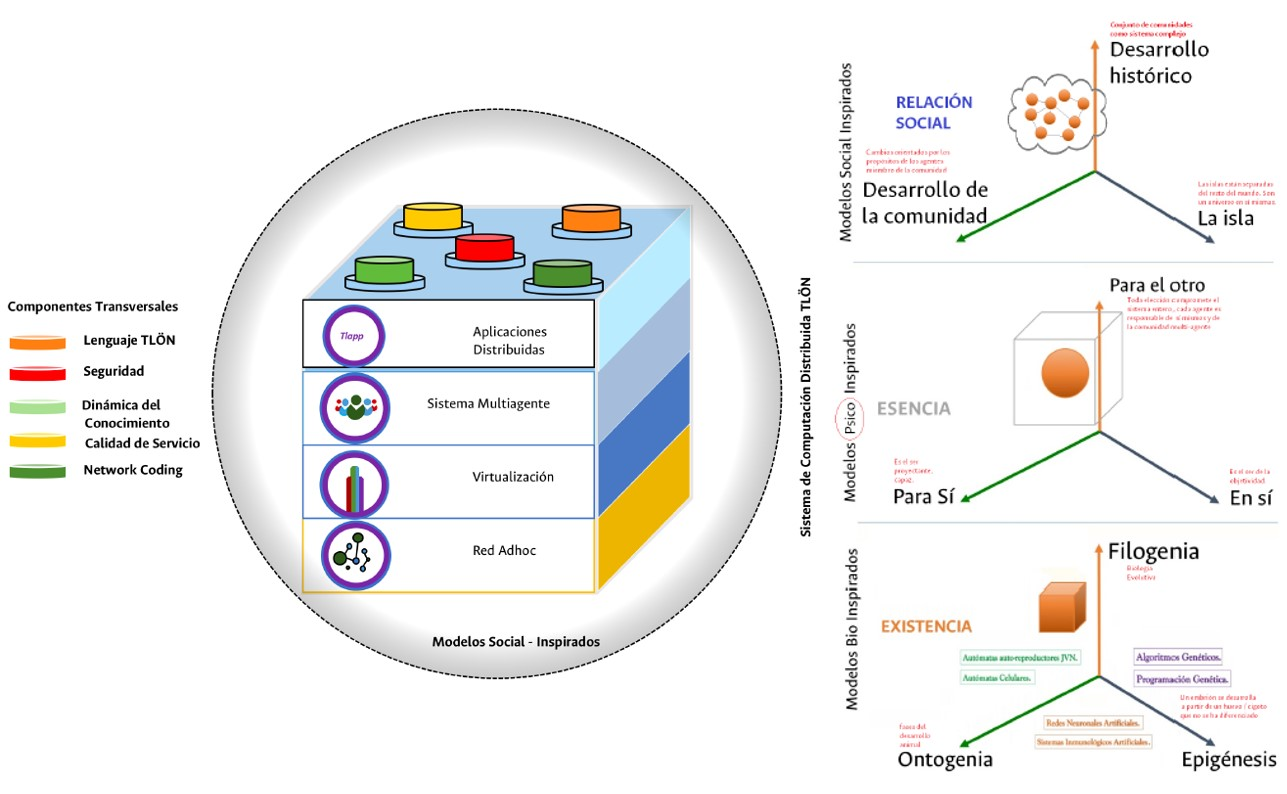
\includegraphics[height=0.55\textheight,keepaspectratio]{Sustentacion/Figures/ModeloTLON2.jpg}}
		\caption{\small \sl Modelo TLÖN}
		\label{figure:TLON}
    \end{figure}
\end{frame}
%-------------------------------------------------------
\subsection{Características}
\begin{frame}{Arquitectura}{Modelo propuesto}
%-------------------------------------------------------
    \begin{figure}				
		\fbox{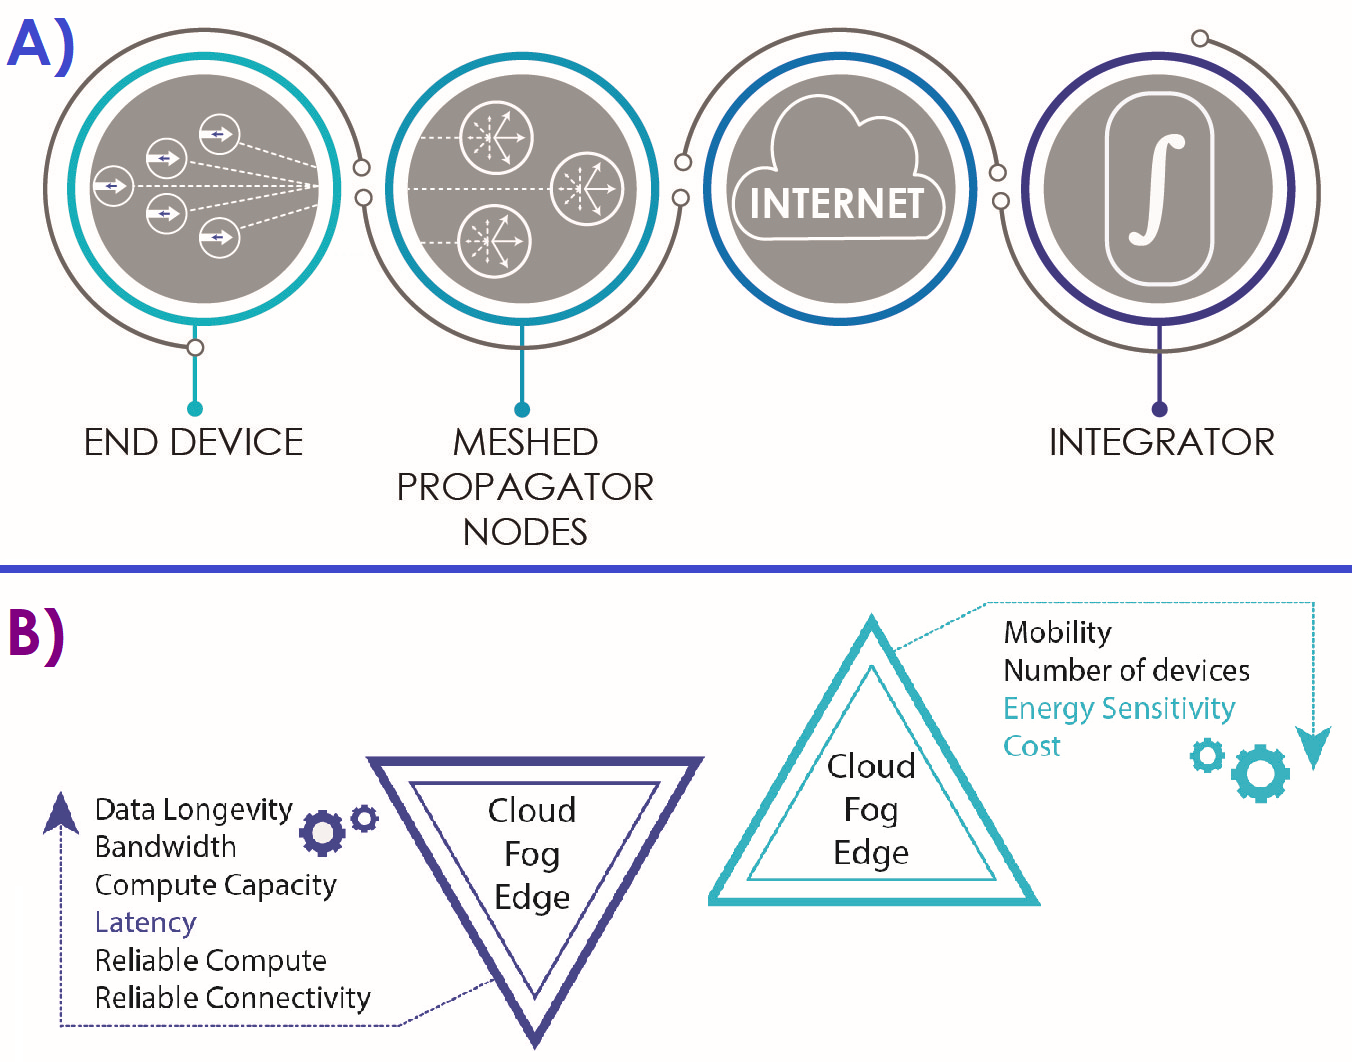
\includegraphics[height=0.68\textheight,keepaspectratio]{Sustentacion/Figures/Arquitectura.png}}
		\caption{\small \sl Arquitectura del modelo \cite{RethinkIOT,MobileEdgeComputing1,MobileEdgeComputing2,FogColony1}}
		\label{figure:Draft}
    \end{figure}
\end{frame}
%-------------------------------------------------------
\begin{frame}{Características - Datagrama e Identificadores}{Modelo propuesto}	
%-------------------------------------------------------
    \begin{figure}				
		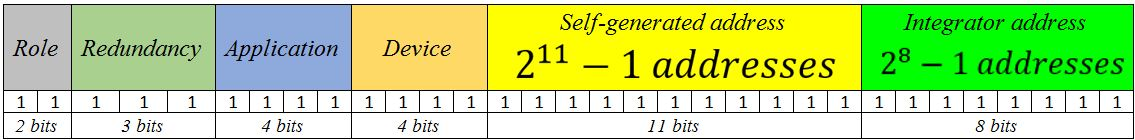
\includegraphics[width=\textwidth,height=0.7\textheight,keepaspectratio]{Figures/Datagram2.JPG}
%		\caption{\small \sl Datagram}
%		\label{figure:Datagram}
%    \end{figure}
%    \begin{figure}		
\\
		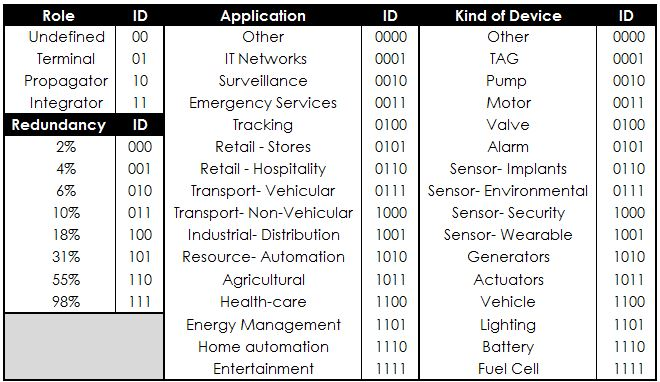
\includegraphics[width=0.85\textwidth,height=0.85\textheight,keepaspectratio]{Figures/IDs.JPG}
		\caption{\small \sl Datagrama e Identificadores externos}
		\label{figure:Identifiers}
    \end{figure}
\end{frame}
%-------------------------------------------------------
\begin{frame}{Características - Modelo matemático}{Modelo Propuesto}	
%-------------------------------------------------------
\begin{align}
AS_{propagator} &= 2^{11+r+a+d}-1  \label{eqn1}\\
AS_{integrator} &= 2^{8+r+a+d}-1  \label{eqn2}\\
Max \# Devices &= AS_{propagator}*AS_{integrator}  \label{eqn3}\\
Min \# Propagator(n) &= \left[ \frac{\# Terminals}{AS_{propagator}} \right ] + \left[D(n)(r+a+d) \right ] \label{eqn4}
\end{align}
Donde:\\
$r$ distintos niveles de redundancia.\\
$a$ cantidad de distintas aplicaciones.\\
$d$ cantidad de distintos tipos de dispositivos.\\
$D(n)$ función de densidad de red en términos del número de nodos.\\
\end{frame}
%-------------------------------------------------------
\subsection{Máquina de Estados Finitos}
\begin{frame}{Máquina de Estados Finitos}	{Modelo Propuesto}
%-------------------------------------------------------
    \begin{figure}				
		\fbox{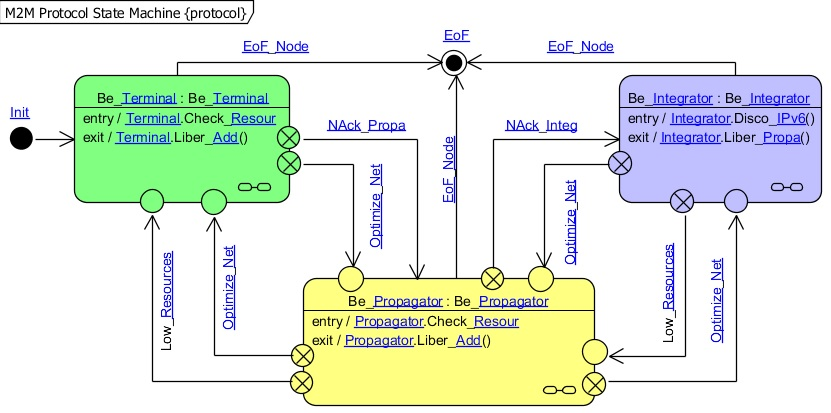
\includegraphics[width=1.0\textwidth,height=1.0\textheight,keepaspectratio]{Figures/M2M_FSM1.jpg}}
		\caption{\small \sl Protocol Finite State Machine}
		\label{figure:ProtocolFSM}
    \end{figure}
\end{frame}
%-------------------------------------------------------
\subsection{Implementación C++}
\begin{frame}{Implementación C++}{Modelo Propuesto}
%-------------------------------------------------------
    \begin{figure}				
		\fbox{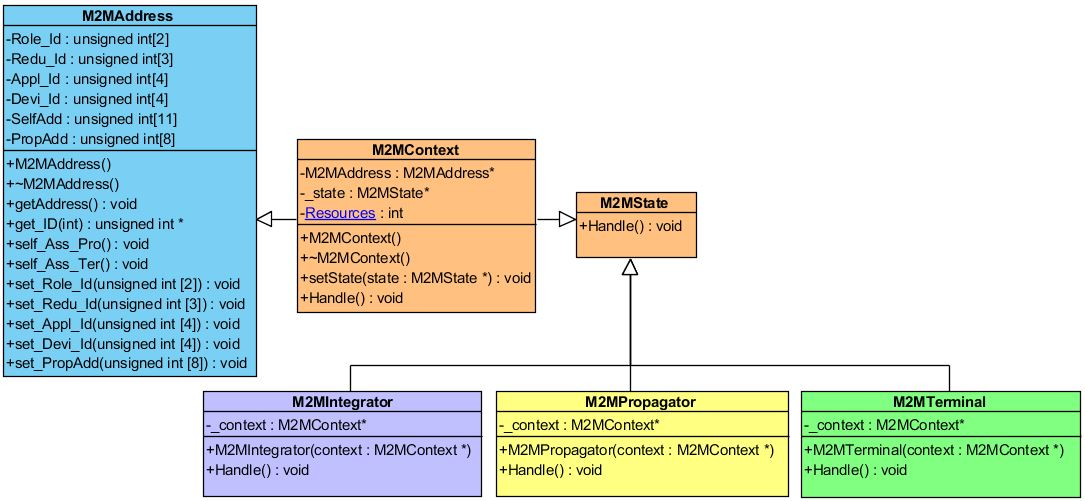
\includegraphics[width=1.05\textwidth,height=1.0\textheight,keepaspectratio]{Figures/DiagramaClases.JPG}}
		\caption{\small \sl Diagrama de Clases}
		\label{figure:DiagramaClases}
    \end{figure}
\end{frame}
%-------------------------------------------------------
\subsection{Implementación NS-3}
\begin{frame}{Implementación NS-3}{Modelo Propuesto}	
%-------------------------------------------------------
    \begin{figure}				
		\fbox{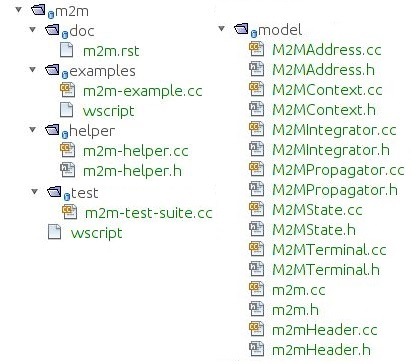
\includegraphics[width=0.6\textwidth,height=1.07\textheight,keepaspectratio]{Figures/NS3.JPG}}
		\caption{\small \sl Librería m2m, disponible: \url{https://github.com/groao/m2m}\\}
		\label{figure:ImplementacionNS3}
    \end{figure}
\end{frame}
%-------------------------------------------------------
	%-------------------------------------------------------
\section{Validación del protocolo}
%-------------------------------------------------------
\subsection{Definición de Métricas}
\begin{frame}{Definición de Métricas}{Validación del protocolo}
%-------------------------------------------------------
\begin{block}{Métricas}
    \begin{enumerate}
    \justifying
        \item \textbf{Uso uniforme} del espacio de direccionamiento \textbf{(UU)}.\\ 
        \item \textbf{Latencia (LA)}: Retardo requerido para la asignación dinámica (setup initial y corrección de duplicidades) \cite{DATMANET}.\\
        {\tt t Latencia promedio por l -saltos\\
        d Diámetro de la red.}\\
        \item \textbf{Overhead (OV)}: Bytes requeridos para establecer el direccionamiento \cite{EvalSelf}\\
        {\tt n Número de dispositivos móviles.\\
        l Número de enlaces.\\
        p Payload.}
    \end{enumerate}
  \end{block}
\end{frame}
%-------------------------------------------------------
\subsection{Escenarios de Simulación}
\begin{frame}{Escenarios de Simulación}{Validación del protocolo}
%-------------------------------------------------------
% \begin{block}{Características escenarios de simulación en NS-3}
%  \begin{itemize}
%    \justifying
%    \item Cantidad aleatoria de nodos (entre 100 y 500), confinados en un espacio de dimensiones finitas.
%    \item La cantidad de recursos computacionales disponibles en cada nodo es asignada según un distribución normal.
%    \item Cada nodo estará dotado de una interfaz inalámbrica de bajo consumo energético. (Zigbee, 6LoWPAN, Wifi, LR-WPAN). 
%    \item Se otorgara movilidad 2D a un porcentaje variable nodos, empleando los modelos $"GaussMarkov2$ y $"Randomwaypoint"$.
%    \item El tráfico característico, es asignado bajo un modelo de $Poisson$. 
%    \item Mediante una distribución aleatoria uniforme, se seleccionan algunos nodos a los cuales se les 'apaga' la interfaz de comunicación.
%    \item Se iteran las simulacionespara identificar si la respuesta general del sistema es mejor debido al 'aprendizaje colectivo'.
%    \item Se somete DHCPv6 a los mismos escenarios.
%  \end{itemize}
% \end{block}
    \begin{figure}				
		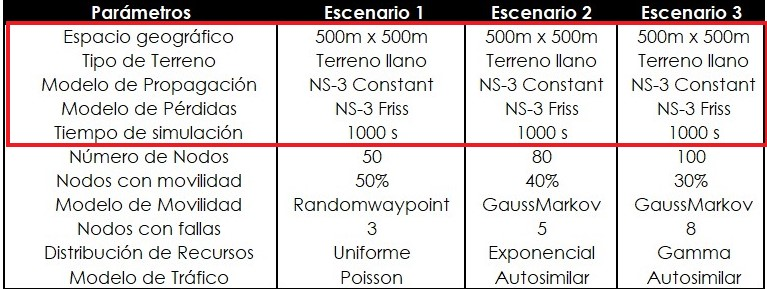
\includegraphics[width=\textwidth,height=\textheight,keepaspectratio]{Figures/ParSim.JPG}
		\caption{\small \sl Escenarios de simulación}
		\label{figure:ParSim}
    \end{figure}
\end{frame}
%-------------------------------------------------------
\begin{frame}{Escenarios de Simulación}{Validación del protocolo}
%-------------------------------------------------------
\begin{align}
RUNS &= l^{(k-p)}  \label{eqn5}\\
fractional_{n!} &= \frac{1}{l^{p}}  \label{eqn6}
\end{align}

Donde:\\
$l$ corresponde a los distintos niveles que puede asumir las variables.\\
$k$ el número de factores o variables estudiadas.\\
$p$ describe el tamaño de fracción del full factorial usado.\\

\begin{align*}
RUNS &= 3^{(6)} = 729  \\
RUNS &= 3^{(6-1)} = 243 => fractional_{n!} = \frac{1}{3^{1}}
\end{align*}
\end{frame}
%-------------------------------------------------------
\begin{frame}{Escenarios de Simulación}{Validación del protocolo}
%-------------------------------------------------------
    \begin{figure}				
		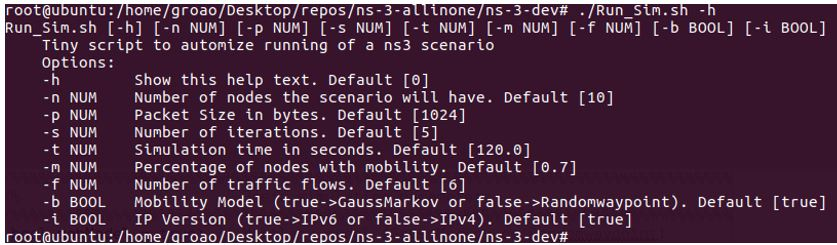
\includegraphics[width=1.\textwidth,height=1.\textheight,keepaspectratio]{Figures/Bash.JPG}
		\caption{\small \sl Bash script}
		\label{figure:Bash}
    %\end{figure}
    %\begin{figure}				
		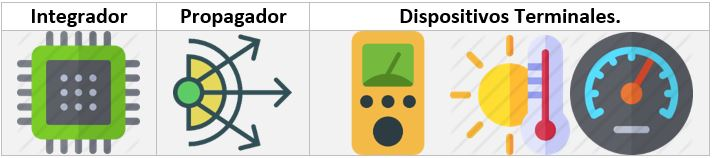
\includegraphics[width=0.8\textwidth,height=0.8\textheight,keepaspectratio]{Figures/Devices.JPG}
		\caption{\small \sl Devices}
		\label{figure:Devices}
    \end{figure}
\end{frame}
%-------------------------------------------------------
\begin{frame}{Escenarios de Simulación}{Validación del protocolo}
%-------------------------------------------------------
	\centering
	\begin{figure}
	%\includemedia[
	    %label=myVidPlayer,
        %width=10cm,height=10cm,
        %activate=pageopen,
    %    addresource=Figures/Avance.mp4,
    %    flashvars={
    %    source=Figures/Avance.mp4
    %    &autoPlay=true
    %    &loop=true
        %&scaleMode=letterbox
    %    },
    %    passcontext
    %]{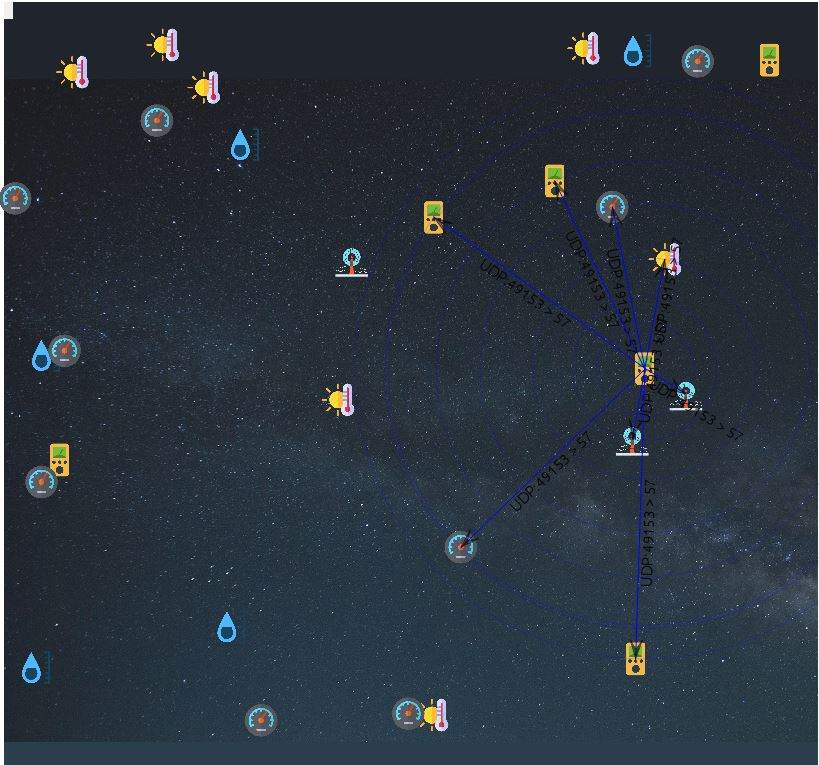
\includegraphics[width=0.8\textwidth,height=0.75\textheight,keepaspectratio]{Figures/Sim.JPG}}{VPlayer9.swf}
    {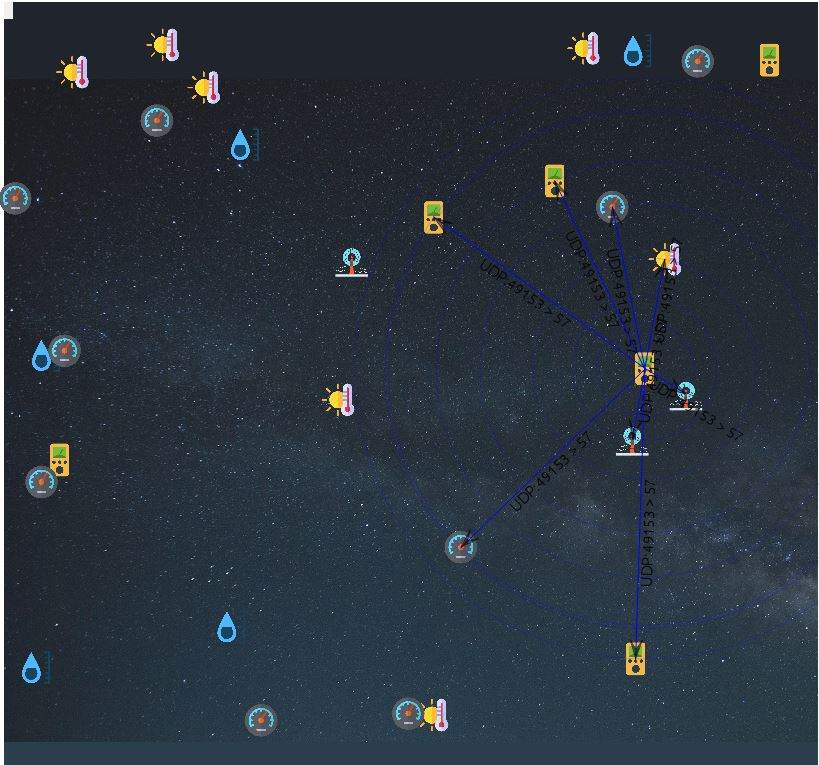
\includegraphics[height=0.75\textheight,keepaspectratio]{Figures/Sim.JPG}}
    \caption{\small \sl Ejemplo Simulación}
	\label{figure:EjemploSim}
	\end{figure}
%-------------------------------------------------------
\end{frame}
%-------------------------------------------------------
\subsection{Resultados}
\begin{frame}{Resultados}{}
%-------------------------------------------------------
    \begin{itemize}
    \justifying
    \item<1-|alert@1> \centering 
\includegraphics[width=0.4\textwidth,height=0.3\textheight,keepaspectratio]{Figures/Tableau.JPG}
    \item<2-|alert@2> Se debe reformular la ecuación (3) \begin{align} Max(\# Devices) &= \left[ AS_{propagator}*AS_{integrator}* \gamma \right ]  \label{eqn7}
\end{align} Donde $\gamma$ corresponde a un factor de seguridad de diseño. Experimentalmente se corroboró que un valor aceptable debe ser máximo \textbf{0.6}.
    \item<3-|alert@3> Se reformula la ecuación (4) \begin{equation}
    %\centering
    Min Propagator(n)=\left\{ \begin{array}{ccc}
            \frac{r+a+d}{D(n)} & n \leq 50 \\
            \\
            \frac{\# Terminals}{AS_{propagator}} + D(n)(r+a+d) & n > 50 
             \end{array}
   \right. \label{eqn8}
    \end{equation}  
  \end{itemize}
\end{frame}
%-------------------------------------------------------
	%-------------------------------------------------------
\section{Conclusiones - Recomendaciones}
%-------------------------------------------------------
\begin{frame}{Conclusiones}
%-------------------------------------------------------
  \begin{block}{Conclusiones}
   \begin{itemize}
   \justifying
    \item<1->  El protocolo recurre a la auto-organización para que la diseminación de paquetes de información sea más eficiente y robusta frente a las dinámicas inherentes de las MANETs.
    \item<1->  Los mecanismos bio-inspirados constituyen, en principio, una opción más eficiente en términos económicos y de complejidad.
    \item<1->  El modelo propuesto reduciría en gran proporción la señalización con respecto a IPv6 ajustándose apropiadamente a las características de las comunicaciones máquina-máquina.
    \item<1->  Delegar tareas de procesamiento y gestión de red hacia los dispositivos ubicados en el "borde" de las redes se plantea como una alternativa efectiva para el despliegue a gran escala del IoT, reduciendo complejidad a la red, mejorando significativamente los tiempos de latencia y blindando a las subredes de posibles vulnerabilidades de seguridad.
    \end{itemize}
  \end{block}
\end{frame}
%-------------------------------------------------------
\begin{frame}{Recomendaciones}
%-------------------------------------------------------
  \begin{block}{Recomendaciones}
   \begin{itemize}
   \justifying
    \item<1->  Este protocolo de direccionamiento puede tener versiones adaptativas emulando efectos vistos en la decodificación del ADN, donde las moléculas poseen fragmentos de información que son activados y sintetizados sólo en ciertas condiciones.
    \item<1->  En aplicaciones reales, la limitación en la cantidad de terminales que pueden ser gestionados por los propagadores estará limitado por los recursos computacionales propios más no por el espacio de direccionamiento. En este sentido es viable sacrificar direccionamiento para modificar el espacio dedicado a los identificadores externos con el fin de hacer cabida a nuevos dispositivos y aplicaciones.
    \item<1-> En el entorno del IoT, los dispositivos de borde podrían aprovechar la infraestructura existente como mecanismo de transporte, es el caso de protocolos como powerline communication. Este tipo de re-usos tendría a su vez un impacto económico muy positivo que aumentaría la masificación del IoT.  
    \end{itemize}
  \end{block}
\end{frame}

%-------------------------------------------------------

\section{Referencias}
\begin{frame}[allowframebreaks]{Referencias} %in case more than 1 slide needed
	
    {\footnotesize
    \bibliographystyle{apalike}
    \bibliography{Reference/IEEE.bib}
    }
\end{frame}

%-----------------------------------------------------

{\4
\begin{frame}[plain,noframenumbering]
    \textbf{\large{\finalpage{\color{white} Gracias por su atención.\\  ¿Preguntas?}}}
\end{frame}}

%-----------------------------------------------------
\end{document}